%% abtex2-modelo-artigo.tex, v-1.9.6 laurocesar
%% Copyright 2012-2016 by abnTeX2 group at http://www.abntex.net.br/ 
%%
%% This work may be distributed and/or modified under the
%% conditions of the LaTeX Project Public License, either version 1.3
%% of this license or (at your option) any later version.
%% The latest version of this license is in
%%   http://www.latex-project.org/lppl.txt
%% and version 1.3 or later is part of all distributions of LaTeX
%% version 2005/12/01 or later.
%%
%% This work has the LPPL maintenance status `maintained'.
%% 
%% The Current Maintainer of this work is the abnTeX2 team, led
%% by Lauro César Araujo. Further information are available on 
%% http://www.abntex.net.br/
%%
%% This work consists of the files abntex2-modelo-artigo.tex and
%% abntex2-modelo-references.bib
%%

% ------------------------------------------------------------------------
% ------------------------------------------------------------------------
%  abnTeX2: Modelo de Artigo Acadêmico em conformidade com
%  ABNT NBR 6022:2003: Informação e documentação - Artigo em publicação 
%  periódica científica impressa - Apresentação
% ------------------------------------------------------------------------
% ------------------------------------------------------------------------

\documentclass[
% -- opções da classe memoir --
article,			% indica que é um artigo acadêmico
11pt,				% tamanho da fonte
oneside,			% para impressão apenas no recto. Oposto a twoside
a4paper,			% tamanho do papel. 
% -- opções da classe abntex2 --
%chapter=TITLE,		% títulos de capítulos convertidos em letras maiúsculas
%section=TITLE,		% títulos de seções convertidos em letras maiúsculas
%subsection=TITLE,	% títulos de subseções convertidos em letras maiúsculas
%subsubsection=TITLE % títulos de subsubseções convertidos em letras maiúsculas
% -- opções do pacote babel --
english,			% idioma adicional para hifenização
brazil,				% o último idioma é o principal do documento
sumario=tradicional
]{abntex2}

\setlength\afterchapskip{\lineskip}

% ---
%  PACOTES
% ---

% ---
% Pacotes fundamentais 
% ---
\usepackage{lmodern}			% Usa a fonte Latin Modern
\usepackage[T1]{fontenc}		% Selecao de codigos de fonte.
\usepackage[utf8]{inputenc}		% Codificacao do documento (conversão automática dos acentos)
\usepackage{indentfirst}		% Indenta o primeiro parágrafo de cada seção.
\usepackage{nomencl} 			% Lista de simbolos
\usepackage{color}				% Controle das cores
\usepackage{graphicx}			% Inclusão de gráficos
\usepackage{microtype} 			% para melhorias de justificação
\usepackage{glossaries}			% solução de glossário
\usepackage{nameref}			% referenciar também pelo nome
% ---

% ---
%  Pacotes de perfumaria
% ---
\usepackage{lipsum}				% para geração de dummy text
% ---

% ---
%  Pacotes de citações
% ---
\usepackage[brazilian,hyperpageref]{backref}	 % Paginas com as citações na bibl
\usepackage[alf]{abntex2cite}	% Citações padrão ABNT
% ---

% ---
%  Configurações do pacote backref
%  Usado sem a opção hyperpageref de backref
\renewcommand{\backrefpagesname}{Citado na(s) página(s):~}
% Texto padrão antes do número das páginas
\renewcommand{\backref}{}
% Define os textos da citação
\renewcommand*{\backrefalt}[4]{
	\ifcase #1 %
	Nenhuma citação no texto.%
	\or
	Citado na página #2.%
	\else
	Citado #1 vezes nas páginas #2.%
	\fi}%
% ---

% ---
%  Configurações do pacote glossaries
\renewcommand*{\glsclearpage}{}
% ---

% ---
%  Informações de dados para CAPA e FOLHA DE ROSTO
% ---
\titulo{Implantação de ligação ferroviária ao longo do curso do rio Tietê na Região Metropolitana de São Paulo: comparação com a infraestrutura existente ao longo do curso do rio Pinheiros}
\autor{Caio César Carvalho Ortega}
\local{São Bernardo do Campo, SP}
\data{06/12/2018}
% ---

% ---
%  Configurações de aparência do PDF final

% alterando o aspecto da cor azul
\definecolor{blue}{RGB}{41,5,195}

% informações do PDF
\makeatletter
\hypersetup{
	%pagebackref=true,
	pdftitle={\@title}, 
	pdfauthor={\@author},
	pdfsubject={Infraestruturas},
	pdfcreator={LaTeX with abnTeX2},
	pdfkeywords={mobilidade urbana}{urbanização}{ferrovia}{infraestrutura}{rios}, 
	colorlinks=true,		% false: boxed links; true: colored links
	linkcolor=black,        % color of internal links
	citecolor=black,        % color of links to bibliography
	filecolor=black,      	% color of file links
	urlcolor=black,
	bookmarksdepth=4
}
\makeatother
% --- 

% ---
%  compila o glossário
% ---
\makeglossaries

% \newglossaryentry{ex}{name={sample},description={an example}}
\newglossaryentry{abl}{
	name={ABL},
	description={Área Bruta Locável}
}

\newglossaryentry{sabesp}{
	name={Sabesp},
	description={Companhia de Saneamento Básico do Estado de São Paulo}
}

\newglossaryentry{bird}{
	name={BIRD},
	description={Banco Internacional para Reconstrução e Desenvolvimento}
}

\newglossaryentry{cptm}{
	name={CPTM},
	description={Companhia Paulista de Trens Metropolitanos}
}

\newglossaryentry{cmsp}{
	name={CMSP},
	description={Companhia do Metropolitano de São Paulo}
}

\newglossaryentry{emtu}{
	name={EMTU},
	description={Empresa Metropolitana de Transportes Urbanos de São Paulo S.A}
}

\newglossaryentry{emplasa}{
	name={Emplasa},
	description={Empresa Paulista de Planejamento Metropolitano S/A}
}

\newglossaryentry{luos}{
	name={LUOS},
	description={Lei de Uso de Ocupação do Solo}
}

\newglossaryentry{mdu}{
	name={MDU},
	description={Média por Dia Útil}
}

\newglossaryentry{ouc}{
	name={OUC},
	description={Operação Urbana Consorciada}
}

\newglossaryentry{pde}{
	name={PDE},
	description={Plano Diretor Estratégico}
}

\newglossaryentry{rmsp}{
	name={RMSP},
	description={Região Metropolitana de São Paulo}
}

\newglossaryentry{ibge}{
	name={IBGE},
	description={Instituto Brasileiro de Geografia e Estatística}
}

\newglossaryentry{gesp}{
	name={GESP},
	description={Governo do Estado de São Paulo}
}

\newglossaryentry{light}{
	name={Light São Paulo},
	description={São Paulo Tramway Light and Power Company Limited}
}

\newglossaryentry{city}{
	name={Cia. City},
	description={City of São Paulo Improvements \& Freehold Land Co. Ltd.}
}

\newglossaryentry{efs}{
	name={EFS},
	description={Estrada de Ferro Sorocabana}
}

\newglossaryentry{pmdi}{
	name={PMDI},
	description={Plano Metropolitano de Desenvolvimento Integrado}
}
% ---

% ---
%  compila o indice
% ---
\makeindex
% ---

% ---
%  Altera as margens padrões
% ---
\setlrmarginsandblock{3cm}{3cm}{*}
\setulmarginsandblock{3cm}{3cm}{*}
\checkandfixthelayout
% ---

% --- 
%  Espaçamentos entre linhas e parágrafos 
% --- 

%  O tamanho do parágrafo é dado por:
\setlength{\parindent}{1.3cm}

%  Controle do espaçamento entre um parágrafo e outro:
\setlength{\parskip}{0.2cm}  % tente também \onelineskip

%  Espaçamento simples
\SingleSpacing

% ----
%  Início do documento
% ----
\begin{document}
	
	% Seleciona o idioma do documento (conforme pacotes do babel)
	%\selectlanguage{english}
	\selectlanguage{brazil}
	
	% Retira espaço extra obsoleto entre as frases.
	\frenchspacing 
	
	% ----------------------------------------------------------
	%  ELEMENTOS PRÉ-TEXTUAIS
	% ----------------------------------------------------------
	
	%---
	%
	% Se desejar escrever o artigo em duas colunas, descomente a linha abaixo
	% e a linha com o texto ``FIM DE ARTIGO EM DUAS COLUNAS''.
	% \twocolumn[    		% INICIO DE ARTIGO EM DUAS COLUNAS
	%
	%---
	% página de titulo
	\maketitle
	
	% resumo em português
	\begin{resumoumacoluna}
		% Instruções do próprio modelo canônico:
		% Conforme a ABNT NBR 6022:2003, o resumo é elemento obrigatório, constituído de uma sequência de frases concisas e objetivas e não de uma simples enumeração de tópicos, não ultrapassando 250 palavras, seguido, logo abaixo, das palavras representativas do conteúdo do trabalho, isto é, palavras-chave e/ou descritores, conforme a NBR 6028. (...) As palavras-chave devem figurar logo abaixo do resumo, antecedidas da expressão Palavras-chave:, separadas entre si por	ponto e finalizadas também por ponto.

		Este artigo tem por objetivo realizar a comparação dos processos de modificação dos rios Pinheiros e Tietê, com vistas à comparação da infraestrutura de transporte sobre trilhos, se propondo a responder se faria sentido implantar uma linha ferroviária ao longo do curso do rio Tietê, de maneira análoga àquela que existe ao longo do curso do rio Pinheiros, fruto da herança da extinta Estrada de Ferro Sorocabana. As bases da comparação objetivada estão calcadas na revisão bibliográfica de teses, bem como dados do poder público correspondentes ao volume de tráfego rodoviário e passageiros no sistema de transporte sobre trilhos.
	
		Destaca-se a assimetria nos processos de retificação dos rios, devido à maior participação da iniciativa privada no caso do rio Pinheiros, bem como a assimetria no próprio uso e ocupação do solo, com grandes empreendimentos imobiliários voltados ao nicho empresarial despontando ao longo do rio Pinheiros.
		
		\vspace{\onelineskip}
		
		\noindent
		\textbf{Palavras-chave}: mobilidade urbana, urbanização, ferrovia, infraestrutura, rios.
	\end{resumoumacoluna}
	
	% ---
	% Título e resumo em língua estrangeira
	% ---
	
	% titulo em inglês
	\titulo{Implementation of a rail link along the course of the Tietê River in the Metropolitan Region of São Paulo: comparison with the existing infrastructure along the course of the Pinheiros River}
	\emptythanks
	\maketitle
	
	% resumo em português
	\renewcommand{\resumoname}{Abstract}
	\begin{resumoumacoluna}
		\begin{otherlanguage*}{english}
			The purpose of this article is to compare the modifying process of the Pinheiros and Tietê rivers, with a look at comparing the mass rail infrastructure, proposing to answer if would make sense to deploy a railway line along the course of the Tietê river, analogous to that one that exists along the course of the Pinheiros river, fruit of the inheritance of the extinct Estrada de Ferro Sorocabana. The bases of the comparison are a bibliographic review of theses, as well as public data from the authorities regarding road and mass rail system passenger traffic volume.
			
			Asymmetry in river rectification processes is highlighted, due to the greater participation of the private sector in the Pinheiros river case, as well as the asymmetry in the land use and occupation, with large real estate ventures aimed at the business niche emerging along the Pinheiros river.
			
			\vspace{\onelineskip}
			
			\noindent
			\textbf{Keywords}: urban mobility, urbanization, railway, infrastructure, rivers.
		\end{otherlanguage*}
	\end{resumoumacoluna}
	
	% ]  				% FIM DE ARTIGO EM DUAS COLUNAS
	% ---
	
	% ----------------------------------------------------------
	%  ELEMENTOS TEXTUAIS
	% ----------------------------------------------------------
	\textual
	\cleardoublepage	% forçar quebra de página (deve violar
						% alguma norma)
	
	% ----------------------------------------------------------
	% Introdução
	% ----------------------------------------------------------
%	\section*{Introdução}
%	\addcontentsline{toc}{section}{Introdução}
%	
%	Preciso verificar se é ou não obrigatório. Mandar mais uma prévia em 6/12 e até 15/12 identifico se preciso ou não escrever uma introdução.
%	
%	\lipsum[3]
	
	% ----------------------------------------------------------
	% Seções do artigo
	% ----------------------------------------------------------
	\section{Elementos estruturadores do território: um histórico} \label{s1:elementos}
	
	% Propósito: realizar uma pequena introdução da seção
	
	A assimetria entre a infraestrutura de transporte existente ao longo do curso dos rios Pinheiros e Tietê, no contexto da \glsdesc{rmsp} e seus processos de urbanização e de uso e ocupação do solo, que conforme \citeonline[p.43]{monteiro2010a}, contribuiu para inserir os dois cursos d'água ``no contexto urbano das últimas quatro décadas, sendo a construção das avenidas marginais, aliada às obras de retificação e canalização, a consolidação dessa atitude''.
	
	Esta seção pretende recuperar os principais elementos do processo histórico, de forma a permitir comparações na \autoref{s1:comparando} (\nameref{s1:comparando}). Serão considerados especialmente o caráter estratégico das várzeas \cite[p.63]{franco2005a} e o ``o papel das ferrovias ao conectar pontos distantes do espaço ocupado pela metrópole'' \cite[p.63]{franco2005a}.
	
	\citeonline[p. 73]{brocaneli2007a} assinala que podemos entendermos as transformações que envolveram os rios Pinheiros e Tietê como fruto da urbanização, industrialização e obras de geração de energia:
	
	\begin{citacao}
		``A transformação da paisagem e da fisionomia dos rios que cruzam o estado de São Paulo está muito mais associada à instalação das cidades, das indústrias e à construção de hidroelétricas com seus respectivos grandes lagos, barragens e eclusas, do que à agricultura que constituiu paisagens nas quais os rios não sofrem grandes interferências, sendo apenas os limites de propriedades.''
	\end{citacao}
	
	\subsection{Rio Pinheiros} \label{s2:riopinheiros}
	
	% Propósito: descrever as intervenções que afetam o Pinheiros
	
	Conforme \citeonline[p. 11]{franco2005a}, a transformação radical da bacia do Pinheiros inicia-se no início do século XX, devido à industrialização crescente. O principal ator responsável por ela é a \glsdesc{light}, de origem canadense. Entre as intervenções realizadas, estava a reversão do curso do rio e sua retificação, de maneira a permitir a drenagem das áreas inundáveis e sua urbanização, antes preterida.
	
	Segundo \citeonline[p. 3]{nobre2000a} a região da marginal do rio Pinheiros é ``a região da cidade que mais tem atraído investimentos na promoção imobiliária de edifícios de escritório desde a década de 70'', outrossim, \citeonline[p. 152]{nobre2000a} também descreve a região da marginal do Pinheiros como sendo o ``local que tem concentrado os megaempreendimentos terciários desde a década de 70'', o que imprime de imediato um papel de destaque para essa parcela do território da metrópole paulista.

	Quando \citeonline[p. 153]{nobre2000a} sumariza os aspectos que levaram à instalação de grandes empreendimentos do setor terciário, elenca: (i) quantidade elevadas de terrenos vagos e de baixo custo na região da marginal do Pinheiros; (ii) acessibilidade devido à importância da próprio sistema de avenidas marginais do mesmo rio, bem como outras avenidas na mesma região e; proximidade com bairros residenciais de alta renda.

%	\subsubsection{Intervenções minoritárias} \label{s3:minoritariaspinheiros}
%	
%	Suprimindo por enquanto.
	
	\subsubsection{O papel da Cia. City} \label{s3:ciacity}
	
	Conforme \citeonline[p. 156]{nobre2000a}, depois da \gls{light}, a \gls{city} (\glsdesc{city}) foi a segunda companhia a atuar na região do rio Pinheiros, fundada em Londres em 1911 e atuante em São Paulo a partir de 1912. Em 1915 a \gls{city} inicia o loteamento do Jardim América, com 1 milhão de m$^{2}$ em formato de bairro-jardim, voltado às classes de alta renda \apud[p. 157]{ottoni1997a}{nobre2000a}. \citeonline[p. 12]{franco2005a} sumariza esta fase da \gls{light} e da \gls{city}:
	
	\begin{citacao}
		``A Cia. Light inaugurou uma nova fase do processo de canalização dos rios e de drenagem das várzeas. Seu projeto não se restringiu apenas à construção da infra-estrutura, mas abrangeu também a urbanização das áreas drenadas, até então alagáveis e portanto preteridas no processo de ocupação urbana. A Light e a \gls{city} foram os principais agentes de urbanização da cidade, responsáveis por projetos rigorosos e qualificados, apesar da perversidade dos meios empregados para atingir os seus propósitos. As atividades dessas empresas implicaram no aproveitamento das várzeas por mais um importante segmento econômico, o capital imobiliário, importante setor numa cidade que sempre teve a sua própria produção como uma de suas principais atividades''.
	\end{citacao}
	
	Nas décadas seguintes, entre 1920 e 1940, a expansão urbana e a especulação imobiliária são fortalecidas com investimentos devido ao capital demasiado acumulado com o crescimento da industrialização, sendo o resultado mais loteamentos, surgidos entre os bairros da Cidade Jardim e Santo Amaro  \apud[p. 157]{langenbuch1971a}{nobre2000a}.  \apudonline[p. 157]{langenbuch1971a}{nobre2000a} destaca as características de tais empreendimentos: ``loteamentos residenciais suburbanos foram sendo criados sem nenhum plano urbanístico, com sistema viário acanhado, de difícil circulação de veículos, com ruas e calçadas estreitas''. Os bairros do Itaim, Vila Olímpia, Campo Belo e Brooklin Paulista surgem neste contexto \apud[p. 157]{langenbuch1971a}{nobre2000a}.
	
	\subsubsection{A construção das vias marginais} \label{s3:construindo}
	
	Todas as rodovias implantadas a partir da década de 1940 convergem para as marginais\footnote{Para \citeonline[p. 157]{franco2005a}, as marginais são ``um conjunto de vias expressas que percorrem um trajeto em paralelo às margens dos rios Tietê e Pinheiros, no trecho que vai da barragem da Penha, ao leste, até o encontro com o Pinheiros, ao oeste, quando então tomam a direção sul em direção à barragem da Guarapiranga''} dos rios Pinheiros e Tietê \cite[p. 12]{franco2005a}, sendo a Anchieta a única exceção. Apesar de terem sido fruto de um grande projeto, \citeonline[p. 12]{franco2005a} salienta que essas avenidas ``são até hoje um gargalo do escoamento da produção do Estado e passagem obrigatória dos fluxos das cargas e de passageiros da metrópole''.
	
	Com relação ao apontamento feito por \citeonline{franco2005a}, especialmente no tocante à questão das rodovias e marginais integradas serem fruto de um ``grande projeto'', cabe reproduzir a diretriz apontada pelo \gls{pmdi} 1970 em \citeonline[p. 16]{gegran1970a}:
	
	\begin{citacao}
		``O sistema de vias descrito seria completado pelas vias metropolitanas que interligariam as vias regionais, assegurando um sistema capaz de suportar o tráfego metropolitano e, ao mesmo tempo, propiciando a criação ou o refôrço de eixos ou centros de atividades.
		
		A principal via com êsse propósito é o Anel Rodoviário que, seguindo a marginal do rio Pinheiros, acompanha o Córrego da Água Espraiada, e segue através do Município de Santo André e inflete na direção Norte até a Via Dutra, nas proximidades de Cumbica. As outras diretrizes são: ligação Via Anhanguera-Itapecerica; Ribeirão Pires-Itaquaquecetuba-Dutra. Ao longo dessas vias, vários núcleos de atividades ou corredores seriam criados para abrigarem atividades industriais, comerciais e serviços.''
	\end{citacao}
	
	A vocação como ``núcleos de atividades ou corredores'', discutida por \citeonline{nobre2000a}, e mencionada na anterior \autoref{s3:ciacity} (\nameref{s3:ciacity}) é flagrante.
	
	\subsubsection{O ramal de Jurubatuba (atual Linha 9-Esmeralda)} \label{s3:linha9}
	
	A gênese do ramal está na visão do engenheiro Asa White Billings, de origem norte-americana, que ao desenvolver o projeto para a retificação e ocupação das várzeas do Pinheiros, vislumbrou também a necessidade de uma nova ligação sobre trilhos entre São Paulo e a Baixada Santista \cite[p. 61]{franco2005a}. Cabe aqui salientar que ``o contrato entre a SPR e o Governo impedia a construção de outras ferrovias em direção ao mar, mas não legislava a respeito de sistemas alternativos'' \cite[p. 61]{franco2005a}. O vislumbre, entretanto, não se mostrou acertado e o ramal não foi bem sucedido devido à pressão da matriz rodoviária.
	
	Há de se considerar que o contexto que levou à construção do antigo ramal de Jurubatuba da finada \glsdesc{efs}, inaugurado em 1957 \cite[p.140]{requena2016a} era distinto e São Paulo apresentava outra configuração populacional, além de pouco dinamismo ao longo do Pinheiros. Segundo \apudonline[p. 157]{langenbuch1971a}{nobre2000a}, o impacto na região foi pequeno, pois ``a área já se encontrava urbanizada e com vocações estabelecidas'', ou seja, a infraestrutura implantada pela \gls{efs} não teve um papel de indução no desenvolvimento urbano, que já havia ocorrido. A principal motivação da Sorocabana foi concorrer com a Santos-Jundiaí e oferecer outra ligação para acesso à Baixada Santista e o Porto de Santos, o que, segundo \citeonline[p.140]{requena2016a}, reduzia a viagem em aproximadamente 80 quilômetros para cargas triadas na Barra Funda. Esta motivação, atualmente, nem mesmo dialoga com o atual uso da Linha 9-Esmeralda do Trem Metropolitano da \gls{cptm}, ao que corroboram trechos dos trabalhos de (i) \citeonline[p.127]{monteiro2010a}: ``o sistema ferroviário, por sua vez, instalado nas várzeas dos dois rios nos primeiros anos de industrialização, é aproveitado posteriormente para o transporte metropolitano'' e; (ii) \citeonline[p.209]{franco2005a}: ``antes majoritariamente destinado ao transporte de cargas, a partir da privatização das ferrovias passou a ser definido como infra-estrutura de interesse prioritário para o transporte urbano de passageiros.'' 
	
	A orientação do planejamento em torno da utilização do ramal pode ser evidenciada quando o \gls{pmdi} prevê novas áreas industriais em regiões consideradas periféricas à época, destacando uma: Santo Amaro: ``ocupando extensa faixa do vale superior do rio Pinheiros com prolongamentos lançados na direção do traçado do Anel Ferroviário'' \cite[p. 8--9]{gegran1970a}. O anel ferroviário mencionado pelo plano é formado, em parte, pelo ramal de Jurubatuba.
	
	Apesar do fracasso, o ramal sobreviveu e deu origem à Linha 9-Esmeralda da CPTM: ``o ramal Jurubatuba permaneceu ocioso na sua função secundária de servir a indústria. Por sofrer a concorrência do modal rodoviário, que se intensificou simultaneamente a sua construção, todo o ramal foi perdendo paulatinamente sua importância'' \cite[p.141]{requena2016a}. Pouco mais de uma década depois de seu surgimento, o ramal de Jurubatuba passa então a ser locus de ações que buscavam dinamizar seu uso:
	
	\begin{citacao}
		``O plano da Fepasa de meados da década de 1970, chamado ``Dinamização da Linha Sul'', consistia em transformar o ramal Jurubatuba num corredor estruturador de alta capacidade de transporte de pessoas, e alimentado pelas linhas de ônibus desviadas das rotas concorrentes para convergirem às estações ferroviárias.'' \cite[p.143]{requena2016a}
	\end{citacao}
	
	\subsection{Rio Tietê} \label{s2:riotiete}
	
	% Propósito: descrever as intervenções que afetam o Tietê
	
	Conforme \citeonline[p. 157]{brocaneli2007a}, o engenheiro Francisco Saturnino de Brito desempenha um importante papel a partir de 1924, quando se torna encarregado da Comissão de Melhoramentos do Rio Tietê, que visava eliminar as cheias do perímetro urbano, permitir a navegação no trecho urbano do rio, afastar a descarga de efluentes \textit{in natura} para jusante do trecho urbanizado e, principalmente: aproveitar a várzea para expansão urbana. Os impactos são notórios: o leito entre a Penha e Osasco é reduzido de 46,3 km para 26 km \cite[p. 158]{brocaneli2007a}, além disso, o sistema viário da cidade, projetado pelo engenheiro Francisco Prestes Maia (Plano de Avenidas) e as intervenções ao longo do rio passam a estar integradas \cite[p. 158]{brocaneli2007a}, sendo que as ideias de Prestes Maia não estavam restritas meramente ao viário, com este apresentando, em 1930, um circuito de \textit{parkways}, inspirado na ideia de um cinturão de parques concebida por Barry Parker em 1919, ainda que não visasse funcionar como cinturão no sentido de barreira contendora do crescimento urbano \cite[p. 158]{brocaneli2007a}.
	
%	\subsubsection{Intervenções minoritárias} \label{s3:minoritariastiete}
%	
%	Suprimindo por enquanto.
	
	\subsubsection{A canalização pelo poder público} \label{s3:canalizacaopub}
	
	Como \citeonline[p. 160]{brocaneli2007a} assinala, as obras de canalização do rio Tietê são iniciadas durante a gestão Prestes Maia, com vistas principalmente à drenagem e apropriação das várzeas como novas terras para exploração, desprezando a memória e identidade da paisagem natural e, ainda que a possibilidade de navegação pelo curso seguisse aventada, o acesso da população ficaria limitado pelas avenidas marginais que acompanhariam o canal. Cabe aqui, entretanto, ressaltar que a exploração das várzeas aterradas não ocorria por falta de áreas de expansão urbana, pois como \citeonline[p. 53]{franco2005a} aponta, ``a oferta de áreas disponíveis município era abundante, de maneira que
	o saneamento das várzeas não representava a única alternativa para o crescimento'', sendo que no caso do Tietê, ainda que o pretexto sanitarista permanecesse, não havia como fortalecer as intervenções com a ideia de geração de energia, como aconteceu com o Pinheiros (vide a \autoref{s2:riopinheiros}). \citeonline[p. 54]{franco2005a} aponta que havia uma conjunção de questões estruturais que permeavam o ideário ligado às intervenções:
	
	\begin{citacao}
		``Tão ou mais importante do que as novas frentes de urbanização, a intervenção nas várzeas equacionava de forma conjunta uma série de questões estruturais: saneamento, drenagem, abastecimento, geração de energia e circulação automotora. Seriam reunidas à ferrovia para ampliar a infra-estrutura básica sem a qual o crescimento, sobretudo industrial, seria insustentável. Entre todos os sistemas implantados, o de transportes desempenharia o papel fundamental de possibilitar a articulação entre os setores produtivos e aglutinar a constelação de bairros definidos por um modelo de ocupação cada vez mais extensivo.
	\end{citacao}
	
	Conforme \citeonline[p. 248]{franco2005a} a canalização do rio Tietê teve como objetivo ``sanear e equacionar o problema das enchentes, que impedia a ocupação efetiva das várzeas'', enquanto as marginais, em convergência, foram um fruto desses esforços, pois ``dependeram dos novos traçados dos rios para ser construídas linearmente''.
		
	Diferentemente do que ocorrera com o Pinheiros, no entanto, as obras envolvendo o rio Tietê não se limitaram a um só ator, nem estiveram ligadas a um único período histórico. Na década de 1970, por exemplo, o poder público seguia planejando e propondo obras de canalização:
	
	\begin{citacao}
		``Construir, a médio prazo, as barragens restantes das cabeceiras do Tietê -- Paraitinga I e III, Jundiaí e Biritiba e executar as obras de canalização e retificação progressiva do Tietê, de jusante para montante, no trecho que se inicia na divisa de Guarulhos com a Capital, na medida em que a ocupação urbana exigir a utilização das áreas marginais alagadiças''. \cite[p. XVIII]{gegran1970a}:
	\end{citacao}
	
	Podemos observar que a ideia de utilização das várzeas continua em voga, bem como a busca por uma divisão funcional do território, esta última identificável pela classificação de áreas na Sub-região Leste da Grande são Paulo com vocação industrial:

	\begin{citacao}
		``Na Sub-região Leste. as áreas planas do vale do Tietê já revelaram aptidão para a. localização industrial e deverão Receber substancial incremento dêsse uso. Sua plena utilização, no entanto, está condicionada à retificação do trecho do rio entre Penha e Mogi das Cruzes, que depende, por sua parte, das obras de regularização em curso no trecho superior do vale.'' \cite[p. 6]{gegran1970a}
	\end{citacao}
	
	Para melhor compreendermos a urbanização ao longo do curso do Tietê, \citeonline[p. 72]{brocaneli2007a} sintetiza a relação entre esta e as infraestruturas rodoviárias e ferroviárias, sendo observável que a infraestrutura rodoviária conduziu a um processo menos racionalizado do ponto de vista da densidade construtiva e do aproveitamento do solo ocupado e em utilização, devido ao caráter de difusão viabilizado por meios de transporte individuais e motorizados:
	
	\begin{citacao}
		``O sistema sobre trilhos significou uma urbanização concentrada ao longo das vias férreas situadas nas várzeas e planícies fluviais, polarizada no entorno das estações e baseada no modal de transporte coletivo. O sistema sobre rodas, fundamentalmente coletivo no primeiro momento, preponderantemente individual com o passar do tempo, possibilitou uma urbanização extensiva, difusa e de baixa densidade''.
	\end{citacao}
	
	\subsubsection{A construção das vias marginais} \label{s3:marginaltiete}
	
	Cabe salientar que o \gls{pmdi} 1970 previa ``concluir a construção do terminal ferroviário de Presidente Altino e promover a construção do terminal sul, junto ao Anel Ferroviário em São Bernardo e do terminal oeste, na Central do Brasil, ao longo da marginal do Tietê'' \cite[p. XVIII]{gegran1970a}. \citeonline[p. 44]{mentone2015a} aponta que o plano ``também previu a localização de indústrias no trecho do rio Tietê entre Penha e Mogi das Cruzes''. As vocações pretendidas podem ser identificada especialmente nos seguintes fragmentos do \gls{pmdi}, separados conforme a sub-região.
	
	Na Sub-região Central previa-se:
	
	\begin{citacao}
		``[\dots] a da Moóca e Ipiranga, estendendo-se linearmente ao longo das linhas da EFSJ; a de Pirituba e Lapa, ocupando os baixos terraços e várzeas da confluência e dos rios Tietê e Pinheiros; a do Belém--Tatuapé, em sua implantação tradicional, sôbre os terraços ferroviários do vale do Tietê; tôdas estas áreas compreendidas nos limites do distrito sede ao município da Capital. Nos demais distritos verifica-se a ocorrência de áreas industriais isoladas, estendendo-se ao longo dos eixos de transporte.'' \cite[p. 9]{gegran1970a}
	\end{citacao}
	
	Na Sub-região Leste previa-se:
	
	\begin{citacao}
		``A localização industrial proposta para esta Sub-região segue um partido principal bem definido, consistente no uso das várzeas, do Tietê. servidas por ferrovia. Dada a natureza do sítio da implantação urbana nestas zonas, as áreas industriais
		se desenvolverão linearmente, intercaladas por áreas verdes ou de usos múltiplos correspondentes aos centros municipais e distritais. Em seu desenvolvimento, são essas áreas acompanhadas pelas localizações em corredor previstas para as áreas comerciais, de forma a propiciar o surgimento de processos de indução mútua e articulação. [...]'' \cite[p. 9]{gegran1970a}
	\end{citacao}
	
	\subsubsection{O Parque Ecológico do Tietê} \label{s3:pet}
	
	\begin{figure}
		\centering
		\caption{Limites do Parque Ecológico do Tietê}
		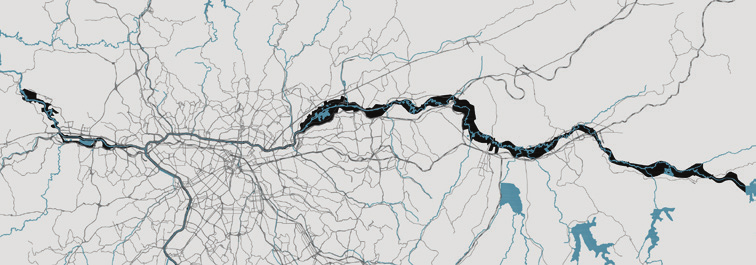
\includegraphics[width=1.0\linewidth]{img/leitao2014_p158a}
		\legend{Elaborado por \citeonline[p. 158]{leitao2014a} a partir de dados de EcoUrbs Ecologia e Urbanismo}
		\label{fig:pet}
	\end{figure}
	
	\citeonline[p. 182]{brocaneli2007a} considera o Parque Ecológico do Tietê, situado a leste da capital e a jusante (vide \autoref{fig:pet} para melhor apreender a localização do equipamento), como um tipo de equipamento escasso na cidade de São Paulo, classificando-o como um espaço urbano no qual ``houve a preocupação da integração do rio com a cidade'' foi no Parque Ecológico do Tietê. Contudo, a integração em questão sofre com as questões previamente apontadas sobre o processo de urbanização e modificação da paisagem do Tietê, apresentando assoreamento devido à baixa velocidade das águas nas lagoas, além de águas contaminadas com material poluente oriundo em grande parte das indústrias situadas no município de Suzano, na Região Metropolitana de São Paulo. \cite[p. 183]{brocaneli2007a} ainda salienta que o Parque Ecológico do Tietê é pouco conhecido e está distante da Zona Central da capital paulista.
	
	\citeonline[p. 111]{leitao2014a} conceitua urbanisticamente o parque linear de 112 km de extensão entre as represas da Ponte Nova e Edgard de Souza, surgido como produto de uma tese que considerava que a continuidade das obras de retificação do rio Tietê abriam a última real oportunidade para criar um parque de dimensões metropolitanas, ou sejas, dimensões substanciais em São Paulo, para se ter uma ideia da grandiosidade do projeto original, `somente a área verde resultante dessa proposta, cerca de 6 mil hectares, já era muito superior à área verde qualificada disponível naquele momento na cidade,	3.200 hectares dispersos'' \cite[p. 111]{leitao2014a}.
	
	\subsubsection{O Parque Várzeas do Tietê} \label{s3:pvt}
	
	Trata-se de projeto desenvolvido por Ruy Ohtake e apresentado em 2009 durante a gestão José Serra do governo paulista, caracterizado por propor a construção de 33 núcleos de equipamentos de esporte e lazer da barragem da Penha ao município de Salesópolis, na \gls{rmsp}. O objetivo do parque seria proteger o rio da ocupação urbana e regular o fluxo das águas, prevenindo enchentes. Ohtake considera que se trata da retomada do projeto do Parque Ecológico do Tietê após mais de 25 anos, embora o aproveitamento do material original dos anos 1970 seja baixo, conferindo identidade arquitetônica distinta \cite[p. 157]{leitao2014a}.
	
	\subsubsection{As diversas linhas do sistema metroferroviário} \label{s3:divferrovias}
	
	Na várzea do Tietê estão presentes uma série de linhas do sistema sobre trilhos, a saber: 3-Vermelha (Barra Funda-Itaquera), 7-Rubi (Luz-Francisco Morato-Jundiaí), 8-Diamante (Júlio Prestes-Itapevi-Amador Bueno), 11-Coral (Luz-Guaianazes-Estudantes) e 12-Safira (Brás-Calmon Viana), sendo a Linha 3 operada pela \glsdesc{cmsp} e as restantes pela \glsdesc{cptm}. A presença das ferrovias, ``principais elementos indutores de desenvolvimento urbano das várzeas'' \cite[p. 247]{franco2005a}, em meio às planícies fluviais não acontece por acaso, pois conforme \cite[p. 247]{franco2005a}, a associação se dá devido às várzeas exigirem pouca intervenção por serem planas, contínuas, desocupadas e de baixo valor.
	
	Em relação à Linha 3-Vermelha, \citeonline[p. 216]{franco2005a} destaca sua sobreposição com os antigos ramais ferroviários que deram origem às linhas da \gls{cptm} citadas no parágrafo anterior:
	
	\begin{citacao}
		``Os primeiros trechos da linha Leste-Oeste, segunda linha 		construída, que viria a ligar a Barra funda com Itaquera, começaram a funcionar em 1979. Essa linha foi sobreposta aos ramais ferroviários presentes na várzea do Tietê e na zona 	leste da cidade, dando novo vigor ao crescimento populacional das áreas ao longo dos	trilhos urbanos, iniciado com os primeiros subúrbio-estação.''
	\end{citacao}
	
	Em relação as linhas da \gls{cptm} que possuem trechos que dialogam com o rio Tietê, \citeonline[p. 224]{franco2005a} destaca a existência de um caráter diferenciado:
	
	\begin{citacao}
		``O trecho compreendido junto às marginais desempenha papel diferenciado, pois, do ponto de vista operacional, é onde se tangenciam e se interligam todas as linhas, gerando alto índice de acessibilidade para essas áreas. Santo Amaro, Berrini, Faria Lima, Pinheiros, Lapa, Barra Funda, Centro, Brás podem ser vistos, desde este ponto de vista, como um colar contínuo e potencialmente articulado das funções de centralidade que já desempenham.''
	\end{citacao}
	
	% ----------------------------------------------------------
	% Estabelecendo comparações
	% ----------------------------------------------------------
	
	\section{Estabelecendo comparações} \label{s1:comparando}
	
	O artigo partiu da premissa de que é possível implantar uma segunda ligação ferroviária, complementar àquela que existe ao longo do curso do rio Pinheiros, descrita na \autoref{s3:linha9}, ademais, é também premissa de que existem políticas e tores consideráveis, assim sendo, faz-se necessário identificar e registrar uma série de elementos, tais como: as principais diferenças na retificação dos dois rios; o volume de tráfego e de passageiros/hora ao longo das vias marginais, de forma a permitir comparações e; identificar o ganho de capacidade possível caso existisse uma linha metroferroviária similar à 9-Esmeralda acompanhando o rio Tietê, incluindo um mapeamento sobre a densidade de conexões e estações por km$^{2}$.
	
	\subsection{Sumarizando as diferenças entre as intervenções nos dois rios} \label{s2:sumarizando}
	
	\citeonline[p. 53--54]{franco2005a} aponta que ``as questões sanitárias eram mais pretextos do que motivos, e a questão energética justificava plenamente as obras do Pinheiros, mas não as do Tietê'', além disso, a retificação foi realizada numa única empreitada e o projeto manteve-se coordenado pela equipe do engenheiro Billings \cite[p. 58]{franco2005a}, e encarregado pela \glsdesc{light}, além disso, a companhia recebeu como compensação o ``direito de desapropriação de todas as terras inundáveis inscritas no limite da maior enchente histórica da qual houvesse registro'' \cite[p. 59]{franco2005a}, sendo que a \gls{light} se voltou à negociação das terras principalmente para a implantação de empreendimentos residenciais de alto padrão \cite[p. 55]{franco2005a}. No caso do outro rio, o poder público foi o responsável pela obtenção de um ``vasto estoque imobiliário na várzea do Tietê, fator que definiria sua ocupação futura pela diversidade de equipamentos, públicos ou privados, assentados sobre áreas de concessão'' \cite[p. 55]{franco2005a}.
	
	Para \citeonline[p. 55]{franco2005a}, ainda que debate ligado à transformação dos dois rios tivesse caráter técnico, nos bastidores desdobrava-se o verdadeiro conflito, ligado à valorização das terras lindeiras ao traçado retificado:
	
	\begin{citacao}
		``Em princípio, questões relativas às retificações começaram a ser pensadas em termos de um processo de apropriação privada do investimento público. Isto porque as várzeas estavam já apropriadas privadamente, tanto as várzeas do Tietê como as do Pinheiros e porque a questão era a de que, através de uma política de investimentos, se faria aplicações de recursos com fins sociais. Não resta dúvida de que pela retificação se realizariam objetivos sociais tanto visando à produção de energia como pela criação de espaços de circulação em que pese o fato desse processo conter, intrinsecamente, inúmeros interesses privados. Pois, é da natureza de todo o processo capitalista de produção da cidade, quer seja através de investimentos públicos ou privados, que tais investimentos alteram de forma substantiva o valor de cada localidade específica. São alterações que respondem positivamente, no seu preço. Um preço que sintetiza uma renda diferencial gerada por essa intervenção''.
	\end{citacao}
	
	Apesar de \citeonline[p. 160]{brocaneli2007a} destacar que as obras de canalização do rio Tietê tiveram caráter urbanístico predatório e pouco contribuíram para o enaltecimento dos recursos naturais como valores ambientais, prejudicando a identidade e a memória da paisagem ambiental, bem como o acesso ao rio pela população e, ainda que intuitivamente se possa pensar que o mesmo venha a se aplicar às obras de canalização do rio Pinheiros, a seguinte constatação de \citeonline[p.148--149]{monteiro2010a} explora a relação paisagística existente, suscitando uma reflexão sobre a diferença entre as infraestruturas ferroviária e rodoviária:
	
	\begin{citacao}
		``Curiosamente, portanto, ainda que se interponha entre o rio e a cidade como mais um elemento de obstáculo ao acesso direto aos rios, a via férrea da CPTM acaba por levar a população às margens dos rios duma outra maneira, ainda que não seja o Pinheiros o lugar de destino intencionado. As estações de trem, nesse sentido, compostas por um edifício de acesso na malha urbana, uma passarela sobre a via expressa e a plataforma, convertem-se em importantes elementos de acesso às mensagens contidas no sistema marginal''.
	\end{citacao}
	
	Ou seja, ainda que não este artigo não tenha como objetivo principal explorar uma relação paisagística que considere uma transformação das margens do rio Tietê a partir da implantação de uma nova infraestrutura ferroviário, pode vir a contribuir para que outros trabalhos desenvolvam-na.
	
	A noção de conveniência sem distinção de renda, melhor compreendida ao observar o que \citeonline[p. 149]{requena2016a} salienta com relação à Linha 9-Esmeralda: ``sua conveniência reside no fato de proporcionar, principalmente ao cidadão de menor renda, meios eficazes de acessar as áreas mais equipadas da cidade para seu uso, independentemente de suas condições financeiras'', trata-se de um atributo inexistente ao longo da Marginal Tietê, na qual o transporte individual motorizado é o principal protagonista como forma de acesso\footnote{Uma reflexão sobre o papel do automóvel em comparação com trens e bondes pode ser conferida em \citeonline[p. 147--149]{franco2005a}.}.
	
	\subsection{Capacidade viária considerando o cenário atual} \label{s2:capacidadeatual}
	
	\subsubsection{Tráfego rodoviário} \label{s3:rodoatual}
	
	\subsubsection{Tráfego rodoviário coletivo} \label{s3:coletivoatual}
	
	\subsubsection{Tráfego metroferroviário} \label{s3:metroatual}
	
	\subsection{Capacidade viária considerando o cenário hipotético} \label{s2:capacidadefuturo}
	
	\subsubsection{Tráfego rodoviário} \label{s3:rodofuturo}
	
	\subsubsection{Tráfego rodoviário coletivo} \label{s3:coletivofuturo}
	
	\subsubsection{Tráfego metroferroviário} \label{s3:metrofuturo}
	
	\subsection{Densidade de conexões e estações} \label{s2:densidadeconexoes}
	
	\subsubsection{Considerando o cenário atual} \label{s3:densidadeatual}
	
	\subsubsection{Considerando o cenário hipotético} \label{s3:densidadefuturo}
	
	% ---
	% Finaliza a parte no bookmark do PDF, para que se inicie o bookmark na raiz
	% ---
	\bookmarksetup{startatroot}% 
	% ---
	
	% ---
	% Conclusão
	% ---
%	\section*{Considerações finais}
%	\addcontentsline{toc}{section}{Considerações finais}
%	
%	Pendente, será trabalhado depois.
%	
	% ----------------------------------------------------------
	%  ELEMENTOS PÓS-TEXTUAIS
	% ----------------------------------------------------------
	\postextual
	
	% ----------------------------------------------------------
	% Referências bibliográficas
	% ----------------------------------------------------------
	\bibliography{fontes}
	\addcontentsline{toc}{section}{Referências}
	
	% ----------------------------------------------------------
	% Glossário
	% ----------------------------------------------------------
	% Consultar manual da classe abntex2 para orientações sobre o
	% uso do glossário.
	\renewcommand{\glossaryname}{Glossário}
	%\renewcommand{\glossarypreamble}{Esta é a descrição do glossário.\\ \\}
	\renewcommand*{\glsseeformat}[3][\seename]{\textit{#1}
		\glsseelist{#2}}
	
	% ---
	% Traduções para o ambiente glossaries
	% ---
	\providetranslation{Glossary}{Glossário}
	\providetranslation{Acronyms}{Siglas}
	\providetranslation{Notation (glossaries)}{Notação}
	\providetranslation{Description (glossaries)}{Descrição}
	\providetranslation{Symbol (glossaries)}{Símbolo}
	\providetranslation{Page List (glossaries)}{Lista de Páginas}
	\providetranslation{Symbols (glossaries)}{Símbolos}
	\providetranslation{Numbers (glossaries)}{Números} 
	% ---
	
	% ---
	% Imprime o glossário
	% ---
	%\cleardoublepage
	\phantomsection
	\addcontentsline{toc}{section}{\glossaryname}
	%\glossarystyle{index}
	\glossarystyle{altlisthypergroup}
	%\glossarystyle{tree}
	\printglossaries
	
	% ----------------------------------------------------------
	% Apêndices
	% ----------------------------------------------------------
	
	% ---
	% Inicia os apêndices
	% ---
%	\begin{apendicesenv}
%		
%		% ----------------------------------------------------------
%		\chapter{Nullam elementum urna vel imperdiet sodales elit ipsum pharetra ligula
%			ac pretium ante justo a nulla curabitur tristique arcu eu metus}
%		% ----------------------------------------------------------
%		\lipsum[55-57]
%		
%	\end{apendicesenv}
	% ---
	
	% ----------------------------------------------------------
	% Anexos
	% ----------------------------------------------------------
%	\cftinserthook{toc}{AAA}
	% ---
	% Inicia os anexos
	% ---
	%\anexos
%	\begin{anexosenv}
%		
%		% ---
%		\chapter{Cras non urna sed feugiat cum sociis natoque penatibus et magnis dis
%			parturient montes nascetur ridiculus mus}
%		% ---
%		
%		\lipsum[31]
%		
%	\end{anexosenv}
	
\end{document}
